\documentclass{article}

\usepackage[utf8]{vietnam}
\usepackage[a4paper, top=2cm, bottom=2cm, left=2cm, right=2cm]{geometry}
\usepackage{booktabs}
\usepackage{amsmath}
\usepackage{graphicx}
\usepackage{scrextend}
\usepackage[fleqn]{nccmath}
\usepackage{setspace}
\usepackage{multicol}
\usepackage{multirow}
\usepackage{fancyhdr}

\pagestyle{fancy}
\fancyhf{}
\rhead{Nguyễn Minh Đăng - 20230022}
\fancyfoot[C]{\thepage}


\setlength{\parindent}{0pt}
\changefontsizes{13pt}
\onehalfspacing


\begin{document}

{
   \setlength{\topmargin}{-0.5cm}
\begin{titlepage}
  \begin{center}
    \centerline{
\includegraphics[height=42mm]{logo}}

    
   \vspace{1cm}

        {\large Trường Đại học Khoa học Tự nhiên}\\[1em]
        {\large Đại học Quốc gia Thành phố Hồ Chí Minh}
    
        \vspace{1.2cm}
    \centerline{\hbox to 13cm{\hrulefill}}
    \vspace{0.3cm}
    \Large  {{Thực Tập Chuyên Đề 1 }}
    \centerline{\hbox to 13cm{\hrulefill}}
    
    \vspace{1.2cm}
    \Large {Bài 9: An Toàn Bức Xạ Ion Hóa Đối Với Bức Xạ Gamma}\\ 
   
   \vspace{3cm}
            \large Người hướng dẫn: Ts. Nguyễn Thị Cẩm Thu \\ 
            \large Sinh viên: Nguyễn Minh Đăng - 20230022
    
    \vspace{4cm}
    

    
    \hbox to \textwidth{\hrulefill}
    \vspace{0.2cm}
    {\sc  04/04/2023}
    
  \end{center}
\end{titlepage}
}

\newpage
\clearpage\thispagestyle{empty}\addtocounter{page}{-1} 
\clearpage
\mbox{}
 % creates a blank space to fill the page
\newpage

\section*{\centering Báo Cáo Kết Quả Thực Nghiệm}

\setcounter{section}{1}

\vspace{0.5cm}

\subsection{Đặt nguồn $\mathbf{{}^{226}Ra}$ vào trong buồng chì chỉ có lỗ chuẩn trực thực hiện phép đo từ xa đến gần các vị trí đo như hình vẽ}

Ta có số liệu như bảng dưới đây
\begin{table}[!ht]
    \centering
    \begin{tabular}{*7c}
    \hline
        \textbf{} & \multicolumn{2}{c}{\textbf{Trung tâm}}  & \multicolumn{2}{c}{\textbf{Trái}} & \multicolumn{2}{c}{\textbf{Phải}}  \\ \hline
        Phông $(\mu Sv/h)$ & d (m) & R1 $(\mu Sv/h)$ & d (m) & R2 $(\mu Sv/h)$ & d (m) & R3 $(\mu Sv/h)$ \\ 
        0,17 & 0,10 & 1100,00 & 0,00 & 6,93 & 0,00 & 6,43 \\ 
        0,14 & 0,20 & 447,70 & 0,10 & 14,20 & 0,10 & 14,57 \\ 
        0,08 & 0,30 & 162,20 & 0,20 & 21,58 & 0,20 & 23,91 \\ 
        0,13 & 0,40 & 73,62 & 0,30 & 25,83 & 0,30 & 25,70 \\ 
        0,11 & 0,50 & 37,73 & 0,40 & 20,53 & 0,40 & 20,74 \\ 
        ~ & 0,60 & 21,17 & 0,50 & 15,59 & 0,50 & 14,51 \\ 
        ~ & 0,70 & 12,20 & 0,60 & 11,34 & 0,60 & 10,93 \\ 
        ~ & 0,80 & 8,10 & 0,70 & 8,05 & 0,70 & 8,39 \\ 
        ~ & 1,00 & 4,38 & 0,80 & 5,91 & 0,80 & 5,99 \\ 
        ~ & 1,50 & 1,20 & 1,00 & 3,46 & 1,00 & 3,87 \\ 
        ~ & ~ & ~ & 1,50 & 1,23 & 1,50 & 1,12 \\ 
        ~ & ~ & ~ & 2,00 & 0,60 & 2,00 & 0,49 \\ \hline
    \end{tabular}
\end{table} \\
Từ số liệu trên ta có đồ thị đã trừ phông

Phải: lấy d từ 0,1 m; trái: lấy d từ 0,3 m; phải: lấy d từ 0,3 m
\begin{center}
	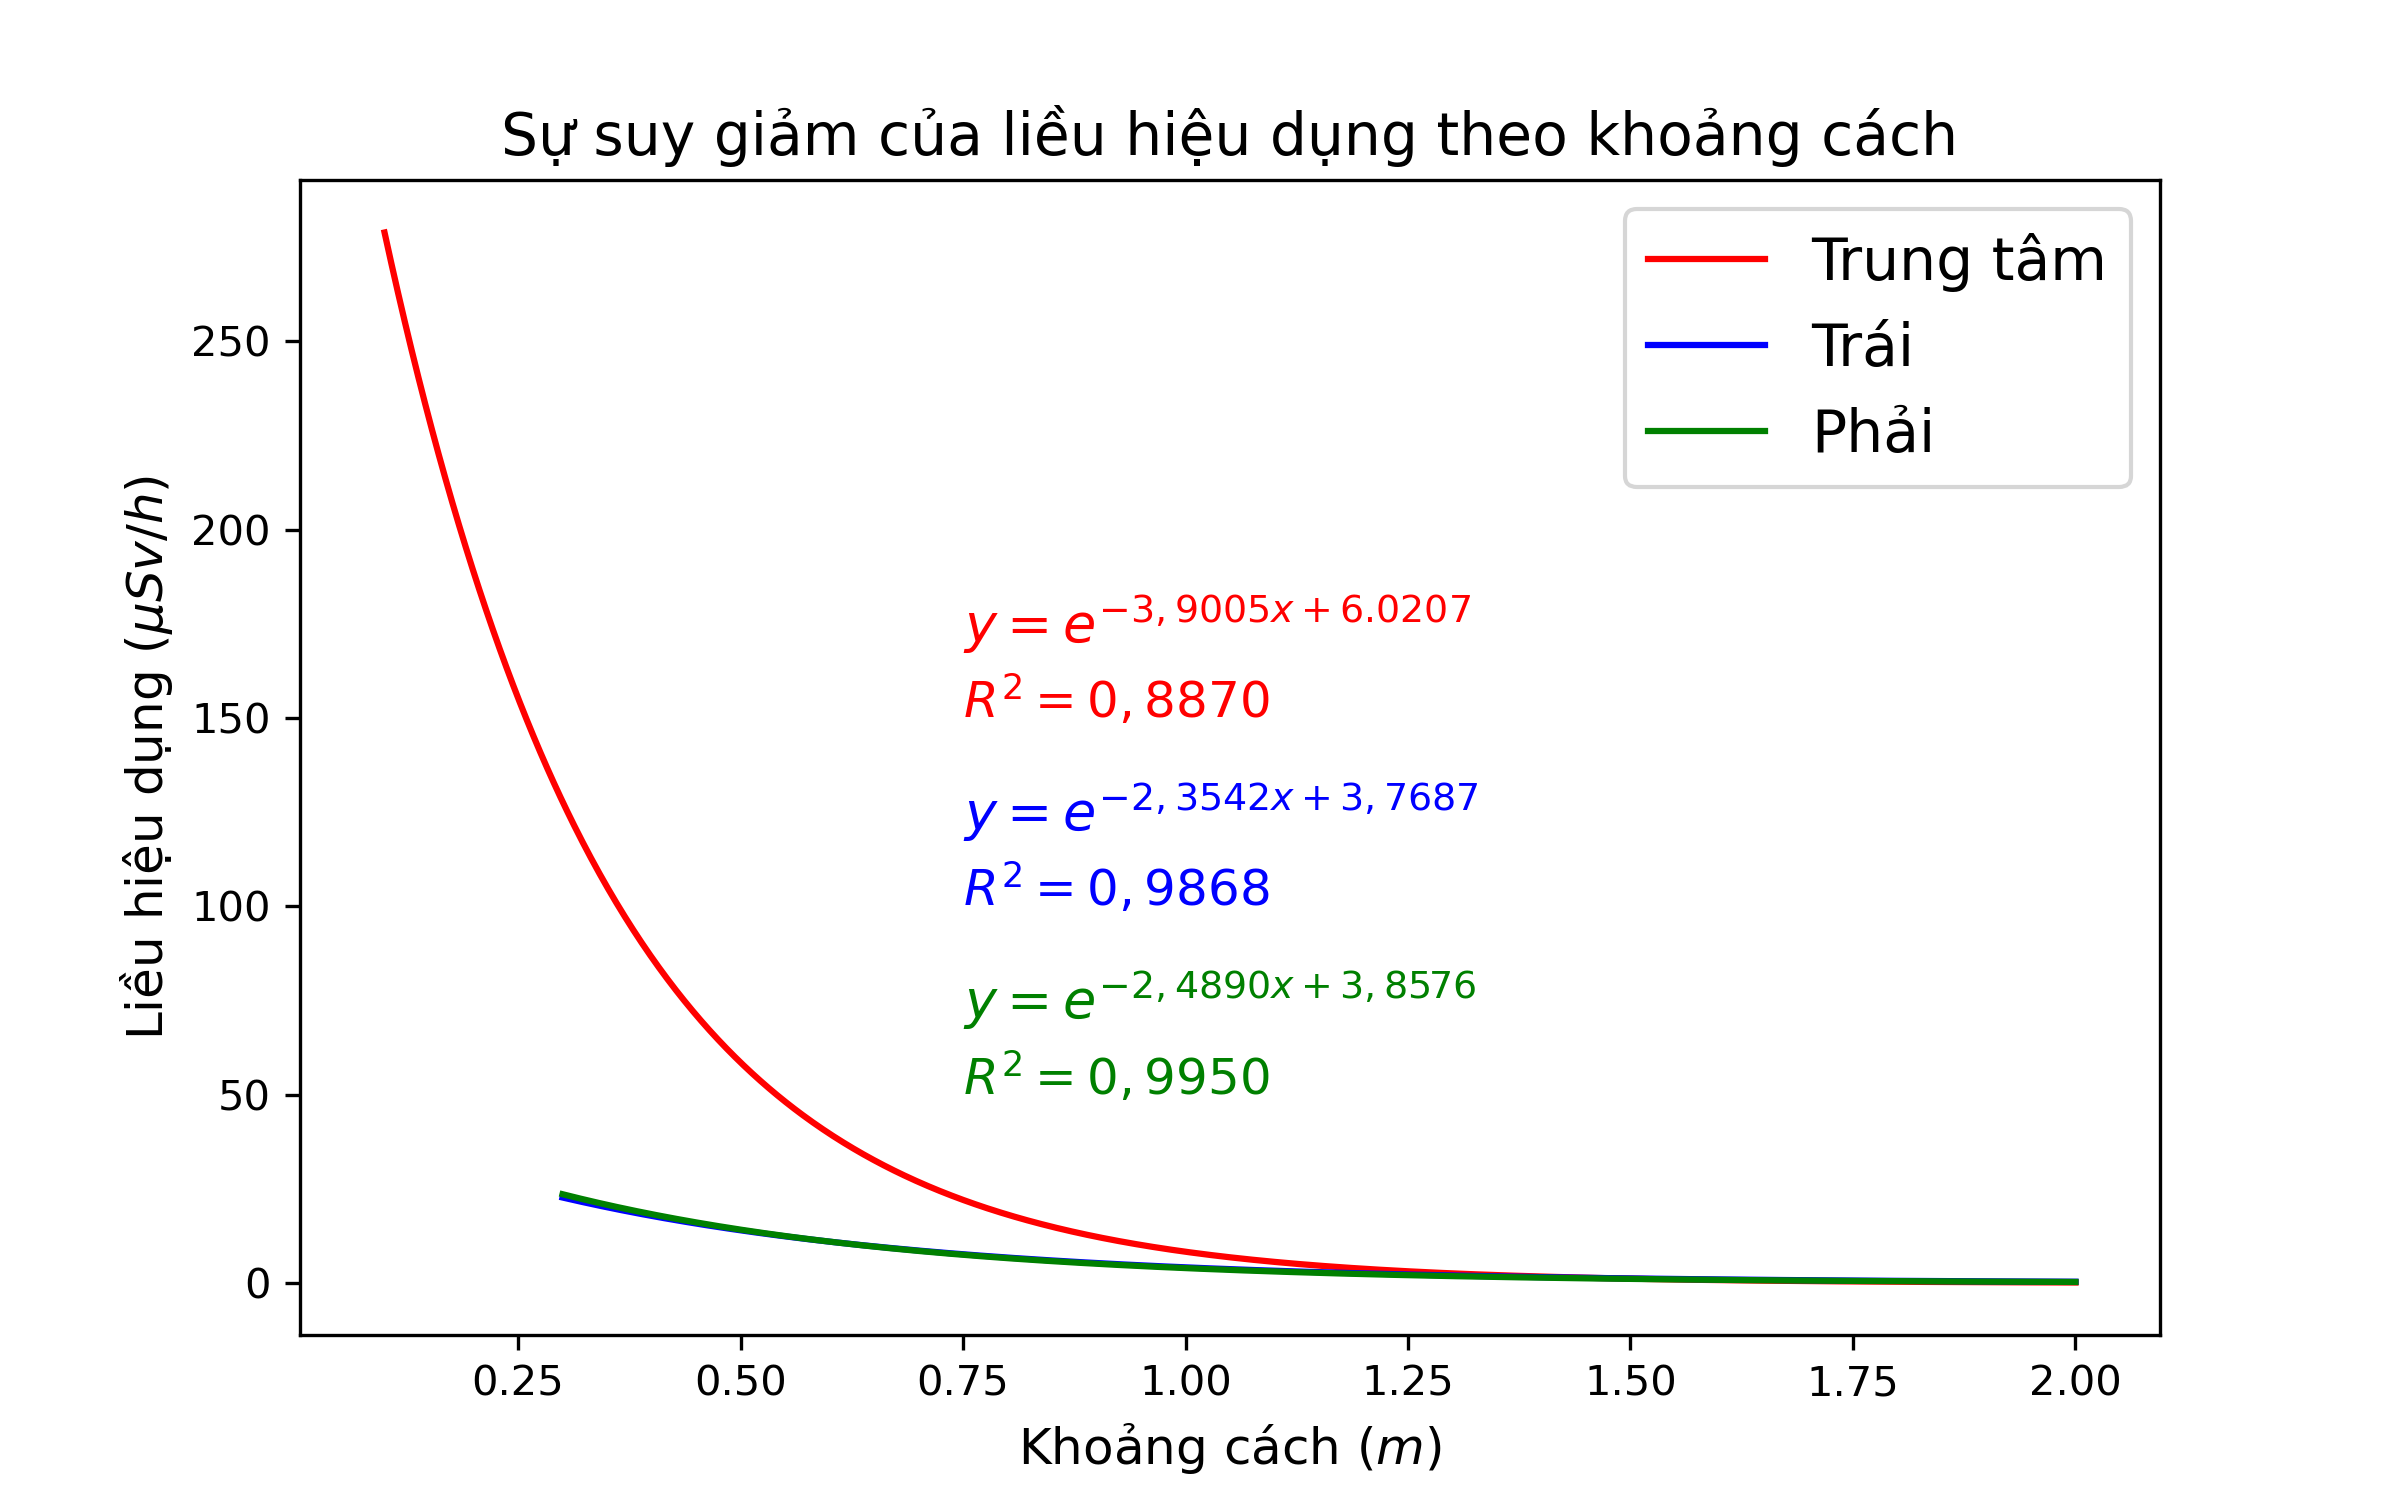
\includegraphics[scale=0.8]{ttb9}
\end{center}
Kết luận: Liều hiệu dụng của nguồn $^{226}Ra$ ở trung tâm sẽ cao nhất, trái và phải ở mức thấp. Nên trung tâm chính diện là nơi nhận được nhiều bức xạ nhất.

\subsection{Nếu giả sử ta có nguồn suất liệu mạnh gấp mười lần suất liều của nguồn này, nếu phải làm việc trong 6 giờ mỗi ngày và không che chắn thì người nhân viên phải ứng cách nguồn gần nhất bao nhiêu để đảm bảo quy tác  an toàn}

Một năm có 365 ngày và nghỉ 2 buổi thứ 7 và chủ nhật, ta có số ngày làm việc $d_w$
\begin{align*}
	d_w = 365 \text{ (ngày)} - \Big(2 \text{ (ngày)} \times 52\text{ (tuần)} \Big) = 261 \text{ (ngày)}
\end{align*}

Mỗi ngày làm việc 6 (h) vậy tổng thời gian $t_{tot}$ làm việc trong 1 năm là
\begin{align*}
	t_{tot} = 261 \times 6 = 1566 \ (h)
\end{align*}

Tiêu chuẩn an toàn là 20 mSv/năm, từ đây ta có liều hiệu dụng tối đa $R_{max}$ trong 1 giờ là:
\begin{align*}
	R_{max} = \frac{20 \times 10^3}{1566} = 12,77 \ (\mu Sv/h)
\end{align*}

Ta có phương trình phương trình hồi quy từ dữ liệu, xét vị trí trung tâm
\begin{align*}
	R = e^{-3,9005x+6,0207}
\end{align*}
\begin{fleqn}[\parindent]
\begin{equation*}
\begin{split}
\text{với : }	& R : \text{Liều hiệu dụng của nguồn} \ (\mu Sv/h)  \\
					& x : \text{Khoảng cách} \ (m)
\end{split}
\end{equation*}
\end{fleqn}

Từ đây ta có khoảng cách tối thiểu $x_{min}$, của một nguồn gấp 10 lần nguồn thử nghiệm
\begin{align*}
	&R_{max} = e^{ax + b} \times 10 \\
	& \rightarrow x_{min} = \frac{ln(R/10) - b}{a} = \frac{ln(12,77/10) - 6,0207}{-3,9005} \\
	& \rightarrow x_{min} = 1,48 \ (m)
\end{align*}

Từ đây ta kết luận muôn an toàn với nguồn mạnh gấp 10 lần nguồn thí nghiệm thì phải đứng xa tối thiểu 1,48 (m)

\subsection{Nếu nhân viên phải đến gần 20 cm hãy tính thời gian tối đa để nhân viên có thể đứng làm việc với nguồn phóng xạ mà vẫn đảm bảo quy tắc an toàn 2 rem/năm}

Theo số liệu thì tại 20 cm ta có $P_{ht} = 447,70$ ($\mu$Sv/h)

Ta có
\begin{align*}
	& P_{ht} = 1 \ (\mu Sv/h) = 0,1 \ (mrem/h) \\
	& \rightarrow P_{ht 20cm} = 447,70 \ (\mu Sv/h) = 44,77 \times 10^{-3} \ (rem/h)
\end{align*}

Vậy số giờ $t_{max}$ tối đa tiếp xúc với nguồn bức xạ này với 20 cm là
\begin{align*}
	t_{max} = \frac{2}{44,77 \times 10^{-3}} = 44,67 \ (h)
\end{align*}

Với nhân viên bức xạ làm việc ngày 6 h thì số ngày tối đa $d_{max}$ tiếp xúc với nguồn bức xạ này trong 20 cm là
\begin{align*}
	d_{max} \approx \frac{44,67}{6} \approx 8 \ \text{(ngày)}
\end{align*}

\subsection{Từ số liệu đo được và áp dụng các công thức trên hãy tính cường độ của nguồn}

Ta có hàm số hàm số gamma ion hóa
\begin{align}
	P = \frac{K_\gamma C}{R^2}
\end{align}
\begin{align*}
	[K_\gamma] = \frac{R.cm^2}{h.mCi} \ ; \quad [R] = Cm \ ; \quad [C] = mCi \ ; \quad [P] = \frac{R}{h}
\end{align*}

Ta xét nguồn tại trung tâm với vị trí có cường độ tại 20 cm, với \\
$P = 447,70 \ (\mu Sv/h)$

Xét mối quan hệ giữa liều chiếu và liều hấp thụ ở không khí
\begin{align*}
	& 1 \ rem = 1 \ rad = 1,14 \ R \\
	& \rightarrow 447,70 \ \mu Sv/h = 44,77 \times 10^{-3} \ rem/h \times 1,14 \ rad/h \\
	& \rightarrow 447,70 \ \mu Sv/h = 0,05 \ R/h
\end{align*}

Từ công thức (1) với $K_\gamma = 8,25 \ R.cm^2/[h.mCi]$, $R = 20 \ cm$, ta có
\begin{align*}
	& C = \frac{PR^2}{K_\gamma} = \frac{0,05\times 20^2}{8,25} \\
	& \rightarrow C = 2,42 \ (mCi)
\end{align*}

\subsection{Giả sử theo đo đạc thực nghiệm P(r) = a/$\mathbf{r^2}$ dùng phương pháp bình phương tối thiểu và bảng số liệu tính các hệ số a. Vẽ đồ thị thực nghiệm và hàm fit của suất liều theo khoảng cách trên cùng một đồ thị. Tìm hàm fit xác định tương đối hoạt độ của nguồn phóng xạ}

Theo đề bài ta có
\begin{align*}
	& P(r) = \frac{a}{r^2} \\
	& ln(P) = ln(a) - 2ln(x) \\
	& \text{ Đặt: } ln(P) = Y; \quad ln(a) = A; \quad 2ln(r) = X \\
	& \rightarrow Y = A - X \\
	& \text{ Đặt: } v_i = A - X_i - Y_i 
\end{align*}

Để tìm điểm cực tiểu, ta đặt
\begin{align*}
	& S = v_i^2 = (A - X_i - Y_i)^2 \\
	& \frac{\partial S}{\partial A} =  \frac{\partial \sum_{i=1}^{n}[A^2 + X_i^2 + Y_i^2 - 2AX_i - 2AY_i - 2X_iY_i]}{\partial A} = 0 \\
	& \rightarrow 2(A - X_1 - Y_1) + ... + 2(A - X_n - Y_n) = 0 \\
	& nA = \sum_{i=1}^{n}X_i +  \sum_{i=1}^{n}Y_i \\
	& \rightarrow ln(a) = \frac{\sum_{i = 1}^{n}2ln(r) + \sum_{i = 1}^{n}ln[P(r)]}{n} \\
	& \rightarrow a = exp\Bigg[\frac{\sum_{i = 1}^{n}2ln(r) + \sum_{i = 1}^{n}ln[P(r)]}{n}\Bigg]
\end{align*}

\newpage
\textbf{Trung tâm}
\begin{table}[!ht]
    \centering
    \resizebox{\columnwidth}{!}{%
    \begin{tabular}{|c|ccccccccccc|c|}
    \hline
        \textbf{} & \textbf{} & \textbf{} & \textbf{} & \textbf{} & \textbf{} & \textbf{} & \textbf{} & \textbf{} & \textbf{} & \textbf{} & \textbf{} & \textbf{Tổng} \\ \hline
        \textbf{ln(r) [m]} & -2.30 & -1,61 & -1,20 & -0,92 & -0,69 & -0,51 & -0,36 & -0,22 & 0,00 & 0,41 & 0,69 & -6,72 \\ 
        \textbf{ln(R1) [m]} & 7 & 6,10 & 5,09 & 4,30 & 3,63 & 3,05 & 2,50 & 2,09 & 1,48 & 0,07 & -0,62 & 35,03 \\  \hline
    \end{tabular}
    }
\end{table}
\\
Theo công thức trên ta có $a_C$
\begin{align*}
	& a_c = exp\Bigg[\frac{2(-6,72) + 35,03}{11}\Bigg] = 7,12 \\
	& \rightarrow P(r)_C = \frac{7,12}{r^2}
\end{align*}

\textbf{Trái}
\begin{table}[!ht]
    \centering
    \resizebox{\columnwidth}{!}{%
    \begin{tabular}{|c|ccccccccc|c|}
    \hline
        \textbf{} & \textbf{} & \textbf{} & \textbf{} & \textbf{} & \textbf{} & \textbf{} & \textbf{} & \textbf{} & \textbf{} & \textbf{Tổng} \\ \hline
        \textbf{ln(d) [m]} & -1,20 & -0,92 & -0,69 & -0,51 & -0,36 & -0,22 & 0,00 & 0,41 & 0,69 & -2,81 \\ 
        \textbf{ln(R2) [uSv/h]} & 3,25 & 3,02 & 2,75 & 2,43 & 2,09 & 1,78 & 1,24 & 0,21 & -0,52 & 16,24 \\  \hline
    \end{tabular}
    }
\end{table}
\\
Theo công thức trên ta có $a_L$
\begin{align*}
	& a_l = exp\Bigg[\frac{2(-2,81) + 16,24}{9}\Bigg] = 3,25 \\
	& \rightarrow P(r)_L = \frac{3,25}{r^2}
\end{align*}

\textbf{Phải}
\begin{table}[!ht]
    \centering
    \resizebox{\columnwidth}{!}{%
    \begin{tabular}{|c|ccccccccc|c|}
    \hline
        \textbf{} & \textbf{} & \textbf{} & \textbf{} & \textbf{} & \textbf{} & \textbf{} & \textbf{} & \textbf{} & \textbf{} & \textbf{Tổng} \\ \hline
        \textbf{ln(d) [m]} & -1,20 & -0,92 & -0,69 & -0,51 & -0,36 & -0,22 & 0,00 & 0,41 & 0,69 & -2,81 \\ 
        \textbf{ln(R) [uSv/h]} & 3,25 & 3,03 & 2,67 & 2,39 & 2,13 & 1,79 & 1,35 & 0,11 & -0,71 & 16,02 \\  \hline
    \end{tabular}
    }
\end{table}
\\
Theo công thức trên ta có $a_R$
\begin{align*}
	& a_l = exp\Bigg[\frac{2(-2,81) + 16,02}{9}\Bigg] = 3,18 \\
	& \rightarrow P(r)_R = \frac{3,18}{r^2}
\end{align*}

\newpage
Từ ba phương trình trên ta có được đồ thị đã trừ phông
\begin{center}
	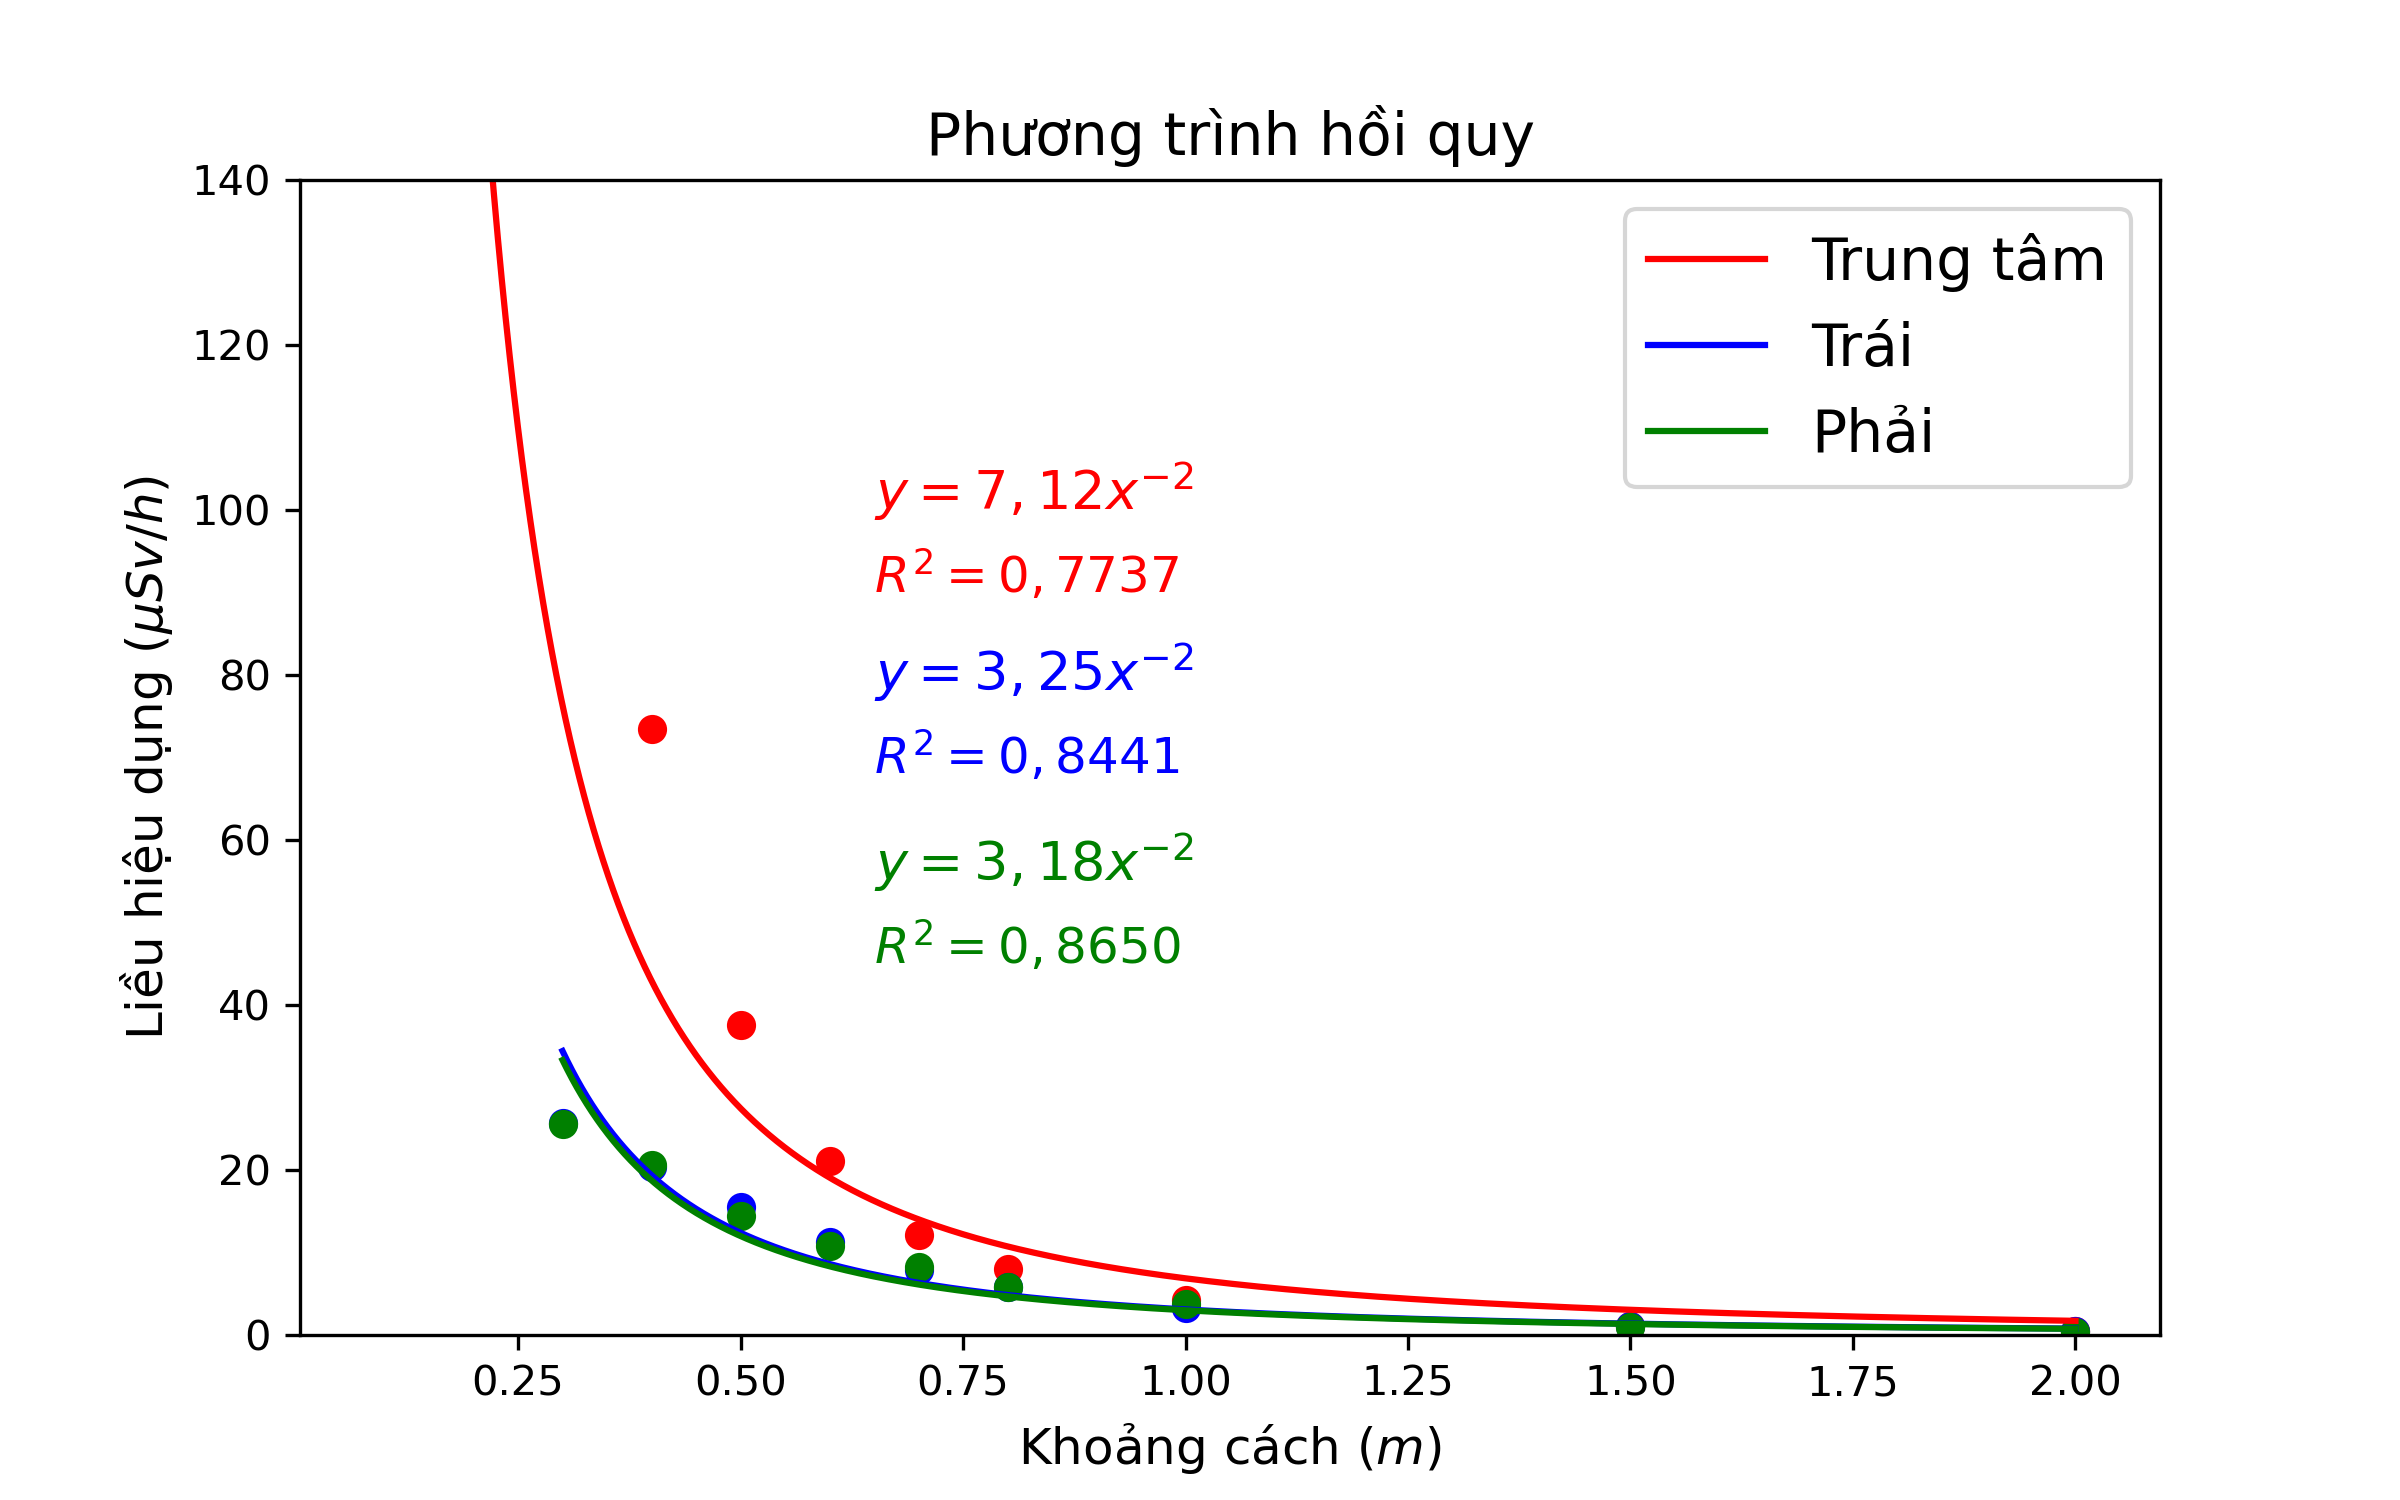
\includegraphics[scale=0.8]{ttb9_b7}
\end{center}

Ta lấy phương trình trung tâm để suy ra hoạt độ
\begin{align*}
	& \rightarrow P(r)_C  \ [\mu Sv/h] = \frac{7,12}{r^2 \ [m]} \\
	& \rightarrow P(r)_C  \ [R/h] = \frac{7,12\times 10^{-4}\times 1,44 \times 10^{-4}}{r^2 \ [cm]} \\
	& \rightarrow K_{\gamma}C = 7,12\times 10^{-4}\times 1,44 \times 10^{-4} \\
	& \rightarrow C = \frac{ 7,12\times 10^{-8}\times 1,44}{ K_{\gamma}} = \frac{ 7,12\times 10^{-8}\times 1,44}{ 8,25 } \\
	& \rightarrow C = 1,25 \times 10^{-8} \ (mCi)
\end{align*}

\newpage
\clearpage\thispagestyle{empty}\addtocounter{page}{-1} 
\clearpage
\mbox{}
 % creates a blank space to fill the page
\newpage


\end{document}